\documentclass[c,unicode,russian]{beamer}
\usepackage{hyperref}
\usepackage{alltt}
\usepackage{verbatim}
\usepackage{fancyvrb}

\usepackage{fontspec}
\setsansfont{Ubuntu}
\setmonofont{Ubuntu Mono}
\usepackage{polyglossia}
\setdefaultlanguage{russian}

\useinnertheme{metropolis}
\useoutertheme{metropolis}
\usecolortheme{metropolis}

\usepackage{listings}   % C++ code
\usepackage{xcolor}     % C++ code
\lstset{%
    keywordstyle=\color{blue},
    commentstyle=\color[rgb]{0.13,0.54,0.13},
    backgroundcolor=\color{yellow!10},
    basicstyle=\small\tt,
    stringstyle=\color{red}\ttfamily,
    belowcaptionskip=-1pt,
    xleftmargin=-15pt,
    framexleftmargin=-15pt,
    framexrightmargin=5pt,
    framextopmargin=5pt,
    framexbottommargin=5pt,
    framesep=0pt,
    rulesep=0pt
}
\lstdefinestyle{cpp}{%
    language=C++,
    morecomment=[l][\color{magenta}]{\#}
}
\lstdefinestyle{python}{%
    language=Python
}

\usepackage{caption}
\renewcommand{\lstlistingname}{Код} % Listing -> Algorithm
\DeclareCaptionFont{white}{\color{white}}
\DeclareCaptionFormat{listing}{\colorbox{gray}{\parbox{\textwidth}{#1#2#3}}}
\captionsetup[lstlisting]{format=listing,labelfont=white,textfont=white}

% logo of my university
\titlegraphic{\hspace{-1cm}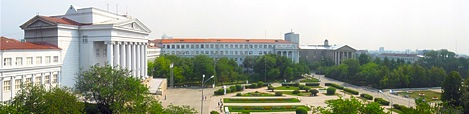
\includegraphics[width=2.5in]{../../_static/logo.jpg}}

\date{}
\author{Основы Веб-программирования}
\institute{Кафедра Интеллектуальных Информационных Технологий, ИнФО, УрФУ}
